%
% Omigost Project
%
% MIT License
% Copyright 2018
%
% Piotr Styczyński     (University of Warsaw)
% Michał Balcerzak     (University of Warsaw)
% Michał Ołtarzewski   (University of Warsaw)
% Gor Safaryan         (University of Warsaw)
%
% Permission is hereby granted, free of charge, to any person obtaining a copy of this software and associated documentation files (the "Software"),
% to deal in the Software without restriction, including without limitation the rights to use, copy, modify, merge, publish, distribute, sublicense,
% and/or sell copies of the Software, and to permit persons to whom the Software is furnished to do so, subject to the following conditions:
%
% The above copyright notice and this permission notice shall be included in all copies or substantial portions of the Software.
%
% THE SOFTWARE IS PROVIDED "AS IS", WITHOUT WARRANTY OF ANY KIND, EXPRESS OR IMPLIED, INCLUDING BUT NOT LIMITED TO THE WARRANTIES OF MERCHANTABILITY,
% FITNESS FOR A PARTICULAR PURPOSE AND NONINFRINGEMENT. IN NO EVENT SHALL THE AUTHORS OR COPYRIGHT HOLDERS BE LIABLE FOR ANY CLAIM,
% DAMAGES OR OTHER LIABILITY, WHETHER IN AN ACTION OF CONTRACT, TORT OR OTHERWISE, ARISING FROM,
% OUT OF OR IN CONNECTION WITH THE SOFTWARE OR THE USE OR OTHER DEALINGS IN THE SOFTWARE.
%
%
%

% Add option for language formatting en/pl
\documentclass[licencjacka,en]{thesisclass}
\usepackage{standalone}
\usepackage{import}
\usepackage{graphicx}
\usepackage{grffile}
\usepackage{svg}
\usepackage{float}
\usepackage{calc}
% json formatting
\usepackage{listings}
\usepackage{xcolor}
\colorlet{punct}{red!60!black}
\definecolor{background}{HTML}{EEEEEE}
\definecolor{delim}{RGB}{20,105,176}
\colorlet{numb}{magenta!60!black}
\lstdefinelanguage{json}{
    basicstyle=\normalfont\ttfamily,
    numberstyle=\scriptsize,
    stepnumber=1,
    numbersep=8pt,
    showstringspaces=false,
    breaklines=true,
    backgroundcolor=\color{white},
    literate=
     *{0}{{{\color{numb}0}}}{1}
      {1}{{{\color{numb}1}}}{1}
      {2}{{{\color{numb}2}}}{1}
      {3}{{{\color{numb}3}}}{1}
      {4}{{{\color{numb}4}}}{1}
      {5}{{{\color{numb}5}}}{1}
      {6}{{{\color{numb}6}}}{1}
      {7}{{{\color{numb}7}}}{1}
      {8}{{{\color{numb}8}}}{1}
      {9}{{{\color{numb}9}}}{1}
      {:}{{{\color{punct}{:}}}}{1}
      {,}{{{\color{punct}{,}}}}{1}
      {\{}{{{\color{delim}{\{}}}}{1}
      {\}}{{{\color{delim}{\}}}}}{1}
      {[}{{{\color{delim}{[}}}}{1}
      {]}{{{\color{delim}{]}}}}{1},
}



\usepackage[backref=true,                %
hyperref=true,               %
firstinits=true,             %
indexing=true,               %
url=false,                   %
style=alphabetic,            %  style=debug, alphabetic
backend=biber,               %
doi=false,
texencoding=utf8,
bibencoding=utf8]{biblatex}

\addbibresource{src/thesis.bib}
\usepackage{biblatex}
\addbibresource{src/thesis.bib}

% Authors of the thesis:
\autor{Piotr Styczyński}{386038}
\autori{Michał Balcerzak}{385130}
\autorii{Michał Ołtarzewski}{382783}
\autoriii{Gor Safaryan}{381501}

\title{AWS Cost Optimization Tool}
\titlepl{Narzędzie do optymalizacji kosztów na platformie AWS}

% The main degree
\kierunek{Computer Science}

% The thesis supervisor
\opiekun{dr Janina Mincer-Daszkiewicz\\
Instytut Informatyki\\
}

% Date in format <month> <year>
\date{June 2019}

% Doctrine of classification as it states the Socrates-Erasmus:
\dziedzina{
11.3 Informatics, Computer Science\\
}

% Subject classification due to ACM
\klasyfikacja{Software and its engineering --- Message oriented middleware\\
    Networks --- Cloud computing\\
    Computer systems organization --- Client-server architectures}

% Keywords list
\keywords{AWS, Amazon Web Services, cloud computing, cost optimization, cost management}

% TODO
% Place for custom definitions and environments
\newtheorem{defi}{Definicja}[section]

% End of definitions

\usepackage{lmodern}

\begin{document}
    \maketitle

    % Brief for the first page (short abstract)
    \begin{abstract}
        %
% AWS Cost Optimization Tool Project
%
% MIT License
% Copyright 2018
%
% Michał Balcerzak     (Univeristy of Warsaw)
% Michał Ołtarzewski   (Univeristy of Warsaw)
% Piotr Styczyński     (Univeristy of Warsaw)
% Gor Safaryn          (Univeristy of Warsaw)
%
% Permission is hereby granted, free of charge, to any person obtaining a copy of this software and associated documentation files (the "Software"),
% to deal in the Software without restriction, including without limitation the rights to use, copy, modify, merge, publish, distribute, sublicense,
% and/or sell copies of the Software, and to permit persons to whom the Software is furnished to do so, subject to the following conditions:
%
% The above copyright notice and this permission notice shall be included in all copies or substantial portions of the Software.
%
% THE SOFTWARE IS PROVIDED "AS IS", WITHOUT WARRANTY OF ANY KIND, EXPRESS OR IMPLIED, INCLUDING BUT NOT LIMITED TO THE WARRANTIES OF MERCHANTABILITY,
% FITNESS FOR A PARTICULAR PURPOSE AND NONINFRINGEMENT. IN NO EVENT SHALL THE AUTHORS OR COPYRIGHT HOLDERS BE LIABLE FOR ANY CLAIM,
% DAMAGES OR OTHER LIABILITY, WHETHER IN AN ACTION OF CONTRACT, TORT OR OTHERWISE, ARISING FROM,
% OUT OF OR IN CONNECTION WITH THE SOFTWARE OR THE USE OR OTHER DEALINGS IN THE SOFTWARE.
%
%
%

The thesis describes the design and implementation process, in-depth system and code architecture
as well as used communication protocols, storing methods and other internals of the AWS Cost Optimization System.
    \end{abstract}

    \tableofcontents

    \chapter{Introduction}

    % 
\includegraphics[width=\textwidth*\real{0.4}]{imgs/logo.png}

    \section{Overview}

    Cloud computing has recently become one of the most significant paradigm shifts
    in the area of real-world software engineering.
    It has reshaped the whole process of how applications are developed
    and reduced the amount of upfront
    investment required to start an internet business.
    While commercial cloud computing services were first offered
    in 2006 by Amazon Inc, the original idea and preliminary
    implementation traces back to Multics OS developed by MIT,
    GE and Bell Labs.
    However the idea of time-sharing systems that was the ancestor of a cloud
    concept was widespread in the 60ies~\cite{Markus}.

    The term \textit{“Cloud computing”} can refer to every layer of application stack:
    hardware, hosting platform, software and even to a single function.
    Cloud computing refers to both the applications delivered as services over the Internet
    and the hardware and systems software in the data centers that provide these services.
    The services themselves have long been referred to
    as \textit{Software as a Service} (SaaS)~\cite{Armbrust}.
    Generally speaking, the cloud can be perceived as a shared pool
    of computer resources such as computing capacity,
    transient and persistent memory, which can be acquired in a form
    of virtual computer instances and then released on demand.
    The undisputed power of cloud computing constitutes
    in its elasticity and granularity: it allows users
    to ask for hundreds of computers for only 5-minute usage which
    are shipped for several minutes.
    Such services are usually offered over a remote network connection and users are billed
    for the portion of the resources, they have used.
    Depending on the cloud infrastructure type the payment models
    can be different~\cite{Laatikainen},
    but the common spendings are associated with data storage,
    data transfer and computing timeshare.

    Nowadays, the industry increasingly relies on cloud technologies.
    More and more companies start or move their products to a cloud environment
    for multiple reasons, including better scalability
    and no need for architecture maintenance.
    Unfortunately, this comes with additional financial costs imposed by cloud providers.
    To make a business profitable, companies try
    to reduce amount of money, they are supposed to pay to the minimum.
    Despite different solutions, like employing specific
    cloud cost optimization team, more and more firms decide
    to benefit from dedicated software, which is supposed to help
    manage and optimize their cloud usage.
    It is not easy to choose the right tool having that many choices.

    There is a number of notable solutions of AWS cloud optimization
    problem -- including \textit{AWS Cost Explorer} and \textit{AWS Cost Management},
    \textit{Cloudability}, \textit{Apptio}, \textit{CloudHealth} -- widely used nowadays.
    In spite of that fact, there is still a place for new tools targeting
    omitted types of clients or wrapping and bundling the most used features from existing ones.
    According to Sumo Logic, the client requesting the software,
    development of which is the main topic of this thesis, there are methods of optimizing costs
    that have the potential to save substantial amounts of money, while the technical details
    of their implementation are not overly complicated.
    Simultaneously, at the moment it seems that there is
    no tool available on the market that approaches the problem
    of AWS optimization in the way that would fulfill
    needs of our client (and other small-to-medium businesses)
    in this simple and cost-optimal way.

    \section{Aim of the thesis}

    The primary objective of the thesis is to create a tool
    complementing existing solutions used in cloud cost optimization.
    We focus on Amazon Web Services platform maintained by Amazon
    as it is one of the most popular cloud service providers.
    In our tool, called \textit{Omigost}, we will try to target small/middle
    sized companies by creating simple and easy to use software
    with flexible configuration options.

    \section{Structure of the thesis}

    The thesis is structured as follows.
    In Chapter 2 we describe the problem of cloud cost optimization.
    Additionally, we review and describe a selection of solutions already available
    on the market.
    In Chapter 3 we present our solution in detail.
    We mention, among others, the system architecture, API and configuration.
    Then, in Chapter 4 we write about our development process -- the tools and techniques
    we used to efficiently communicate and coordinate with people involved in the project
    and successfully deliver the product.
    Finally, in Chapter 5 we sum up the whole thesis.
    In Appendix A we describe how to introduce our solution in a company.

    \section{Contribution of each author}

    It is essential to mention that each author worked to some extent on every part of the thesis.
    However, the authors contributed mainly to the following parts throughout the project:

    \begin{itemize}
        \item Michał Ołtarzewski
        \begin{itemize}
            \item software development process management
            \item design of backend architecture
            \item implementation of Slack API connection
            \item backend part implementation
        \end{itemize}
        \item Michał Balcerzak
        \begin{itemize}
            \item research of existing solutions
            \item design of backend architecture
            \item implementation of budget overflow notifications
            \item backend part implementation
        \end{itemize}
        \item Piotr Styczyński
        \begin{itemize}
            \item design and prototype of a visual part of the tool
            \item localstack integration
            \item AWS deployment automation
            \item frontend part implementation
        \end{itemize}
        \item Gor Safaryan
        \begin{itemize}
            \item research of AWS APIs and SDKs
            \item design of backend architecture
            \item implementation of machine termination flow
            \item backend part implementation
        \end{itemize}
    \end{itemize}

    \section{CD contents}
    To this thesis is attached a CD disc with the source code of the project.
    The most important parts of the code are split into three main folders:
    \begin{itemize}
        \item `frontend` containing React frontend
        \item `server` with Spring backend
        \item `deployment` containing scripts for deploying the application
            both locally and via Elastic Beanstalk (an AWS cloud service
            for deploying applications)
    \end{itemize}
    Every main component of the project is described in
    `README.md` files placed in the corresponding folders.

    \chapter{Problem statement}

    \section{Motivation}

    As there is plenty of various billing models for cloud services~\cite{Laatikainen},
    the effective management of them became a severe problem.
    The ease of resource allocation led to a situation where tracking all of
    the tiniest details of the billings is an unaffordable challenge.

    However, according to our client, some businesses the client is in contact with
    (as well as himself) reported demand for a tool that would provide budgeting management
    and basic machine termination automation.
    Such a tool may not cover as many use cases as the tools
    available on the market, but it would allow for huge savings while
    also being simple in implementation and maintenance.
    The tooling that exists is targetting wide world-scale companies
    that can require expensive licenses and hire cost-optimization teams.

    This is a demand in the small-to-medium business market that our solution,
    \textit{Omigost}, attempts to cover.
    Having one versatile tool removes the need for using a few detached pieces of software.
    The most important aspects of our tool are an intuitive interface and a variation
    of user notifications, which highly increase spendings clarity
    and help in decisions related to costs cutting.
    We hope it will allow companies to focus more on providing value to their clients
    and have significantly lower costs at the same time without having to spend resources
    on an extensive toolkit for cost optimization.
    This should be possible to achieve with budget and machine termination solutions
    that are very simple in concept and implementation, but still provide significant savings.

    During the designing process of Omigost, we decided to dedicate our
    attention to providing a solution with the following features:
    \begin{itemize}
        \item free and open source
        \item easy cloud management without complex knowledge
        \item intuitive interface for individual workers to request resources
        \item notifications for cost surpassing and redundant resources
        \item proper notification management -- only significant alerts
        \item integration with communication via Slack
    \end{itemize}

    \section{Overview of exisiting solutions}

    Businesses that rely upon cloud services often reach a point where resources
    they are using up gradually become less and less manageable.
    As the problem is well known to the cloud market, both Amazon
    and other third-party companies made attempts to fulfill these needs
    by creating custom software implementing various AWS expense optimization approaches
    that include:

    \begin{enumerate}
        \item budget limit configuration, alerting users when those are exceeded
        \item instance alerting management
        \item cost analytics
    \end{enumerate}

    Some of the most prominent tools currently available
    on the market that improve resource management experience
    for AWS cloud are described in the following sections.
    Every description is supposed to show key features crucial for cost optimization.

    \subsection{AWS Budgets}

    AWS Budgets~\cite{AWSDocs} is a part of Amazon Web Services that allows
    to limit how many resources of a certain type are used on AWS
    throughout a selected period (i.e. every month).
    AWS enables its users to specify the scope of such a budget in detail.
    For example, one may make a budget only consider costs of those machines
    that are either tagged in a specific way
    or are owned by a defined group of accounts.

    When a limit is either exceeded, close to being exceeded or is forecasted
    to exceed the configured threshold before the end of that period,
    a preconfigured action takes place.
    For such an occasion, the administrator can either choose
    to have email notifications sent out to a list of addresses
    or have Amazon's Simple Notification System (SNS) triggered.
    SNS provides the AWS users a way to implement custom notification flows.

    Types of resources one can put this kind of a budget on include:

    \begin{enumerate}
        \item money spent in total or on a certain type of machines
        \item utilisation of selected services
        \item utilisation or coverage of reserved instances
    \end{enumerate}

    \subsection{AWS Cost Explorer and AWS Cost Management}

    AWS Cost Explorer~\cite{CostExplorer} enables access to all budget data.
    User can define and generate custom reports in a form
    of a data chart spanning a selected time interval
    with chosen time granularity of the samples.
    AWS Cost Explorer is also a basis for AWS Cost Management,
    which is a set of predefined reports
    that form an easily accessible dashboard.
    % https://aws.amazon.com/aws-cost-management/

    \subsection{Cloudability}

    Atlassian's Cloudability~\cite{Cloudability} delivers
    a budget system functionality analogous to AWS Budgets
    along with tools for predicting future spendings
    and presenting the real cost of AWS resources in utilisation.
    In comparison to Amazon's native tools, Cloudability
    also allows management of multiple accounts at the same time.
    It saves the effort of having to set up budgets separately in every owned account.

    \subsection{Apptio}

    Apptio~\cite{Apptio} provides a set of tools that mainly focuses on analysis
    of expenses and their forecasts,
    managing them collaboratively and planning future ones.
    They expose features that make it easier to discover underutilized resource,
    compare spendings with a database of similar benchmarks,
    organize resources into groups to make reports even clearer,
    and offer other useful management utilities.

    \subsection{Stax.io}

    Stax.io's~\cite{Stax.io} main focus is to provide insight about cost,
    wastage, compliance and cloud quality.
    It can analyse how cloud resources are used, measure quality of the way cloud is utilized,
    set up checks for business-compliance of a cloud with several standards
    and give customized advice on what could be optimized to reduce wastage,
    while also allowing for creation of custom views of data.
    Essential tools for budgeting instances, accounts, tags and more, monthly or annually,
    and configuring overspend alerts are also available there.

    \subsection{SnowSoftware}

    SnowSoftware's toolset, alongside fulfilling some of the more specific use cases,
    like optimizing usage of software from SAP Software Solutions or optimizing
    and managing software licenses,
    also has tools that are dedicated to optimizing cloud costs.

    Snow for SaaS attempts to give a holistic view about application usage
    including, among others, how SaaS applications are used
    on cloud and whether there are zombie virtual machines~\cite{SnowSaaS}.

    Snow Automation Platform suggests an approach based on automated
    and preconfigured provision of resources.
    By pre-giving these resources a decommission date one can avoid the issue of zombie instances.
    It is also possible to preconfigure budgets and schedule machine starts
    and stops to further optimize costs~\cite{SnowBlog}.

    \section{Conclusions}

    The research we made based on the resources that
    are publicly available on the Internet.
    Although we did not have sufficient resources to see
    the tools we are considering here in practice,
    the resources allowed us to conclude that most of the competing tools
    available on the market don't target simpler use cases that could
    cover basic optimization needs of smaller businesses
    that rely on AWS cloud.

    Instead, the creators of such toolkits often
    focus on delivering multifaceted and highly configurable systems.
    Such tools are an overkill for the optimization needs of the small-to-medium
    businesses.
    These tools often require costly subscriptions and lots of time
    to understand and configure them.
    Many of them also fail to provide features
    that allow for both instance budgeting and machine termination automation.
    A number of them puts most of their emphasis on analysing
    usage data rather than helping with instance management.

    Our research failed to find a tool that would be a close match to the needs
    of businesses similar to our client's.
    From among the tools listed in section 2.2, Snow Automation Platform
    is the only system that features both budgeting and automating
    machine termination.
    However, its approach is not to straightforwardly manage
    already existing machines,
    but rather to automate their provisioning.
    Incorporating this kind of a flow in our client's company would
    require multiple changes in the way the developers use the AWS cloud
    and the compound cost of both a restructurization and
    a subscription fee is not worth it when compared to the idea of Omigost.

    In some cases, the software, as it is in case of Cloudability
    and the toolset provided by AWS, is too complex and low-level
    for an average user in a day to day usage.
    While covering those specific budgeting and termination needs
    would be possible, it would require lots of time spent
    on research, configuration and maintenance.

    Cloudability~\cite{CloudabilityAlerts} offers simple alerts, but they lack
    Slack (team collaboration toolkit, communication service) support
    and beforementioned termination abilities.
    Tools provided by Amazon also don't have any out-of-the-box
    Slack integration.
    They rather provide basic building blocks that Omigost uses
    to implement handling of the budgeting and termination
    use cases of our client.
    Amazon doesn't provide a complete service
    that would provide them.

    \chapter{Tool for AWS cost optimization}

    In this chapter, we describe the application \textit{Omigost}.

    \section{Our solution}

    Omigost is an application that focuses on two main tasks:
    \begin{enumerate}
        \item easily manageable AWS Budgets; and
        \item automatic machine termination.
    \end{enumerate}

    It uses Slack integration as a convenient and not overly intrusive mean
    of providing employees a simplified way of saving a company's money in their day-to-day work.

    \section{Use cases}

    In this section, you can find the descriptions of the most common use cases
    grouped by the system actors.
    Every use case assumes that the company is already
    preconfigured in AWS Organizations.

    \subsection{Actor -- AWS cost optimization administrator}

    Administrator is somebody who has an access to the Omigost AWS Cost Optimization platform.
    Most of the interactions happen through the application website.

    First of all, the administrator can configure users inside the application.
    Using the configuration tab, the administrator can:

    \begin{enumerate}
        \item Add an employee.
        \item Add a contact to an employee (currently only Slack).
        \item Link an account to a specific employee.
        \item Define a timeframe for when the system should suggest machine termination.
    \end{enumerate}
    It is important to mention that most of the similar
    actions, like editing and deleting, are also possible.

    Apart from the configuration, an administrator can have an insight
    into AWS costs by looking at dashboards with charts.
    It is also possible to customize charts to show only subset of costs.

    \subsection{Actor -- Employee}
    An ordinary employee does not have access to the platform itself.
    Most of the interactions happen through Slack.
    There are a few situations when a user can receive Slack messages from an application bot:

    \begin{enumerate}
        \item Budget has been surpassed.
        \item Budget is forecasted to being surpassed.
        \item Machine on AWS works in timeframe specified for machine termination.
    \end{enumerate}

    If any of the budgets linked to the employee's accounts are surpassed,
    the employee will receive a notification.
    Additionally, if a budget has a machine tag filter configured,
    account owners of those machines that surpass that budget will be notified.

    Messages sent by the bot are rather simple.
    They consist of a title, a button and a description that includes
    information about a triggered budget.
    Clicking the button redirects to a dedicated form website on our frontend
    which allows the employee to request more money from the manager.

    \bigskip

    We can imagine the following example scenario:
    \begin{enumerate}
        \item A budget is being surpassed.
        \item The employee receives a message from the bot on Slack.
        \item The employee analyzes the description.
        \item The employee decides to request more money and clicks the button.
        \item The employee is redirected to the request form website.
        \item The employee completes and submits the request form.
    \end{enumerate}

    \bigskip

    The situation with machine termination is very similar.
    If a machine linked to the account owned by the employee
    is found to be running in a defined timeframe, a notification will be triggered.
    The message body contains a machine description, a stop button and a termination button.
    By clicking one of these buttons, the user can conveniently
    stop or terminate the corresponding machine without having
    to enter AWS' interface dedicated for that purpose.


    \section{Overall architecture}

    \begin{figure}[H]
      \center{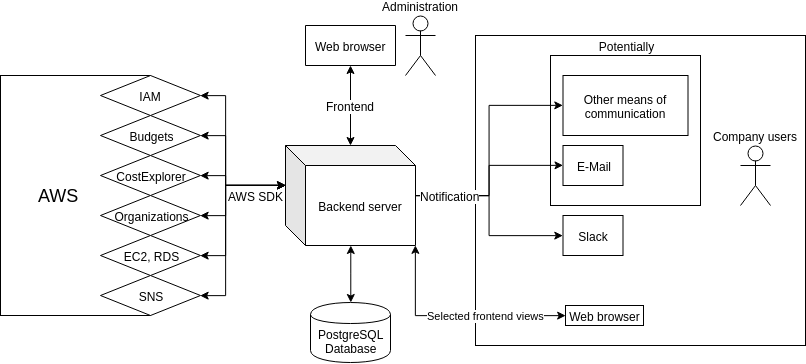
\includegraphics[width=\textwidth,height=200pt,keepaspectratio] {imgs/arch_diagram.png}}
      \caption{Draft diagram of the tool architecture\label{fig:arch-diag}}
    \end{figure}

    Our solution is based on an architecture that is visualized on Figure 3.1.

    The architecture of the tool can be described as traditional client-server architecture.
    Actors make requests over the HTTP protocol to the system with a web browser
    using the frontend client application
    served by the Omigost server or from any storage
    service like, for example, Amazon's S3.
    Those requests are then handled by a backend application running on a central server machine.
    During the handling process, our application uses both a local instance
    of a PostgreSQL relational database
    and a connection with selected Amazon Web Services via an SDK library.
    Additionally, end users are notified about budgets
    and reminded about instances termination through Slack.

    \subsection{Role of AWS cloud services}
    Connecting with Amazon's cloud services not only allows the application
    to access machine and spending data,
    but many of them also solve many of the problems we would otherwise have
    to explain ourselves -- resulting
    in time saved and a codebase that is more concise and easier to maintain.

    Services that are used in the project and their respective roles in it are as follows:
    \begin{itemize}
        \item Identity and Access Management (IAM) -- the provision of the main
          Amazon account ID that is used in other services
        \item Organizations -- insight into the structure of the Organization
          used by the company, including listing accounts
        \item Budgets -- a service monitoring spendings that triggers
          a SNS notification whenever a budget limit is or is going to be exceeded
        \item SNS -- alert notifications for the backend that let it know about spending events
        \item Cost Explorer -- data for graph visualization of the spendings in the frontend
        \item EC2/RDS -- information about the state of the instances running on the account
    \end{itemize}

    \subsection{Backend}

    The backend is the main agent of our application's functionalities.
    It is responsible for fetching or receiving data from either
    of other connected resources, parsing it and taking appropriate actions.
    Some of its more important tasks include:
    \begin{itemize}
        \item receiving SNS budget alert notifications
          and notifying appropriate users via Slack,
        \begin{itemize}
            \item providing single-use tokens and links
              that allow non-administrator users to interact with the system,
        \end{itemize}
        \item fetching and providing raw data for the frontend
          so it can be displayed to the user,
        \item receiving configuration or data modification requests
          and adjusting the application environment components to fulfill them,
        \item checking the machine state on preconfigured times
          and notifying users about possible instance optimizations.
    \end{itemize}

    \subsection{Frontend}
    The frontend is a web application that allows the user to see
    and alter the state of the application using a graphical user interface (GUI).
    Its main roles are to:
    \begin{itemize}
        \item request and parse raw data from backend into visual representations of it;
        \item provide an interface for the user; and
        \item translate the interface clicks to appropriate backend requests
          and display the results of these requests.
    \end{itemize}

    \section{Technology stack}

    \subsection{Frontend}

    The frontend was written in the Typescript~\cite{Typescript} language
    using the React~\cite{React} framework.
    Typescript offers both great flexibility and type safety compared to vanilla Javascript.
    It is the most common alternative to Javascript,
    supported by large business institutions, like Microsoft.
    We decided that other alternatives,
    i.e. Reason (or other functional languages compiled to Javascript) or Dart are useful,
    but still need development and their interoperability is sometimes a very limiting factor.
    All the codebase is linted using \textit{tslinter}.

    The Typescript code is transpiled
    using \textit{tsc} and bundled by \textit{webpack}.
    We do not use any other build tools, like
    \textit{Grunt} or \textit{Gulp}, as the backend has its own tooling, i.e. Gradle.
    It would just unnecessarily complicate the building process without any gains.
    The frontend build is coordinated by an npm plugin for Gradle.

    The frontend codebase is split between universal,
    reusable components
    and concrete implementation of user views.
    That design decision was an effect of the general good programming guidelines.
    It enables future application contributors and users
    to effectively implement customizations or modification
    in existing code without unnecessarily big work efforts.

    The views are split between various \textit{modules}.
    A module is a standalone entity that provides its
    own button in the sidemenu of the application.
    For increased customizability and modularity, each of them
    can be separately disabled or modified.
    To synchronize the data between the separate modules we decided
    to use \textit{Redux} with its Flux architecture.
    This allows us to easily persist the application state
    in the local storage of the browser or elsewhere.
    The Redux store is a central storage for the information
    about current module settings but also serves view routing data,
    state of dialogs and notifications.

    \subsection{Backend}

    The core of the backend is \textit{Java 8}.
    We have selected this programming language because most of us were familiar with it.
    Also, this language has a huge community and lots of useful libraries and frameworks.

    For the creation of the complete backend service, we have chosen Spring~\cite{Spring} framework.
    It is currently one of the most common choices.
    Spring allows building web applications imposing usage
    of design patterns, like Model-View-Controller and Dependency Injection.
    It helps to keep the code easily testable and well organized.
    Additionally, it provides various features out of the box,
    and this speeds up the development process.

    Gradle~\cite{Gradle} is responsible for build and dependency management.
    It is easy to use with various IDEs and has a flexible configuration.
    The main competitor of Gradle is Maven so we have considered both.
    For us, Gradle turned out to be the better choice because
    of its performance and user convenience.

    For data persistence, we have chosen a PostgreSQL database.
    A relational database enforces to have a strictly defined data model with validation.
    The performance is not that much of an essential aspect for us here
    so there was no need for any other type of a database.
    PostgreSQL is a great open source database with strong data integrity
    and fault-tolerance guarantees.
    Furthermore, AWS allows to set up PostgreSQL instances with just a few clicks
    with parameters that are automatically configured for optimal performance.

    In our application we use the following libraries:
    \begin{enumerate}
        \item Spring Core, Spring Boot, Spring Data, Spring Web,
        \item Project Lombok,
        \item JUnit,
        \item AWS SDKs.
    \end{enumerate}

    \subsection{Deployment}

    The whole tool is bundled up by Docker.

    Following a straightforward instruction, everyone is able
    to create their own Docker image of the application.
    Moreover, all of the configuration is present in one file,
    making it easy to adapt it in one's way.

    A preferable method of deployment is to use the AWS Elastic Beanstalk with a Docker image.
    In such a way AWS will be responsible for almost everything,
    including capacity provisioning, load balancing and auto-scaling.

    \section{Views and design}
    
    \subsection{General design}
    
    The main design principles that we used in application design and implementation were:
    \begin{enumerate}
        \item Interface usability is more important than its look.
        \item The style should be as simple and minimalistic as possible.
        \item Use limited color pallete with few colours that match each other perfectly.
    \end{enumerate}
    
    The Omigost icons were drawn in Inkscape as SVG graphics and we created primitive,
    initial mocks in UXPin \cite{UXPin} tool.
    
    \subsection{Login view}
    
  
    The login view (Figure 3.2) is designed with geometric simplicity in mind.
    It is showing the Omigost basic color palette basing mostly on red, which we consider
    a default main color that can be associated with the main application logo.

    \begin{figure}[H]
      \center{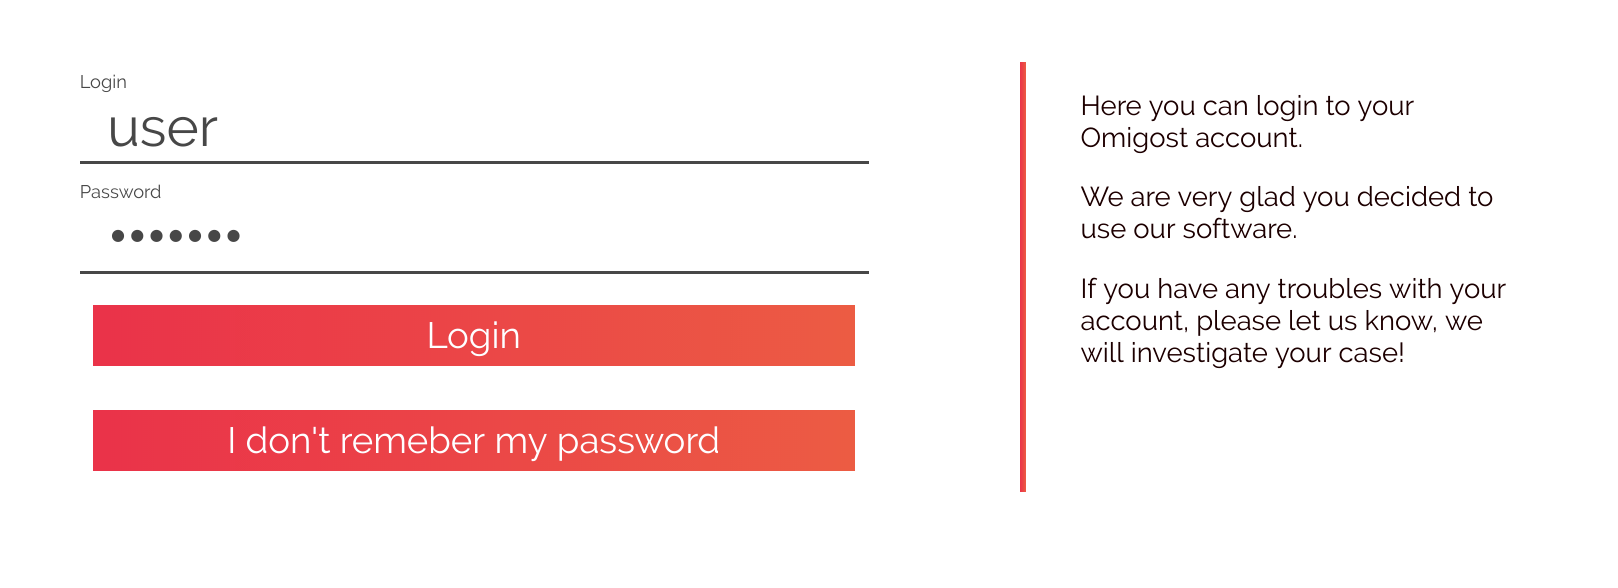
\includegraphics[width=\textwidth,height=200pt,keepaspectratio] {imgs/screenshots/screen_login.png}}
      \caption{The login screen\label{fig:scr-login}}
    \end{figure}
    
    \subsection{Dashboard}
    
    The very first user experience after the login screen and the loading screen is the dashboard (Figure 3.3).
    Here you can add customized widgets to display the AWS costs data.
    A simple interface (Figure 3.4) allows users to select and add new widgets
    and configure them in any way desired by the user.

    \begin{figure}[H]
      \center{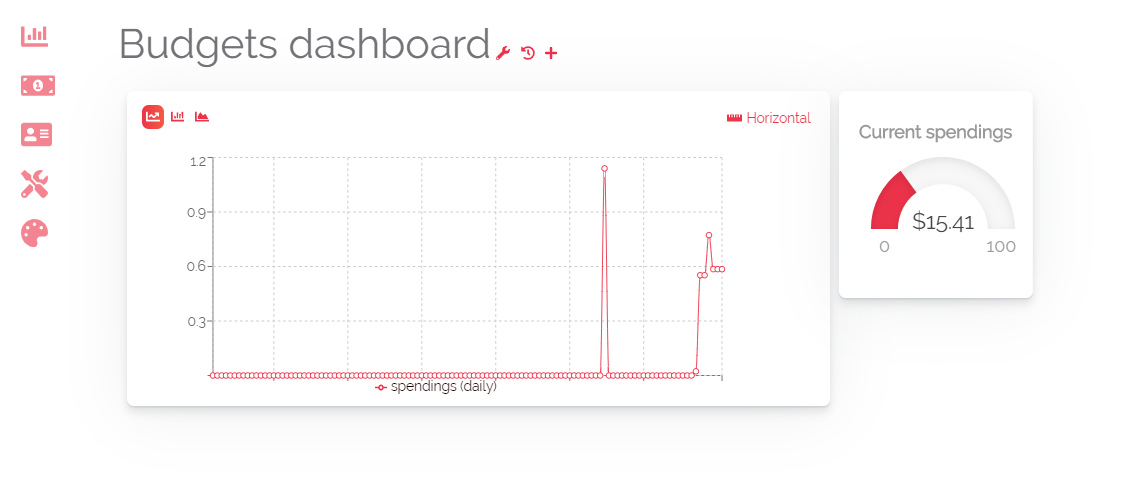
\includegraphics[width=\textwidth,height=200pt,keepaspectratio] {imgs/screenshots/screen_dashboard.png}}
      \caption{The dashboard\label{fig:scr-dashboard}}
    \end{figure}

    \begin{figure}[H]
      \center{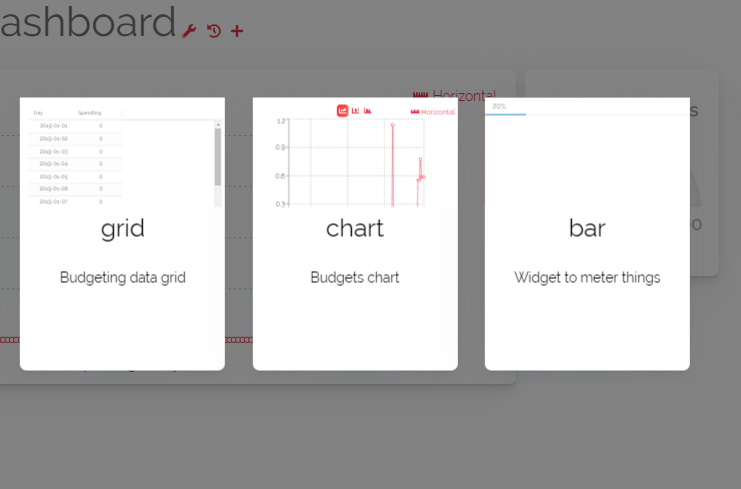
\includegraphics[width=\textwidth,height=200pt,keepaspectratio] {imgs/screenshots/screen_dashboard_add.png}}
      \caption{Adding widgets to the dashboard\label{fig:scr-dashboard-add}}
    \end{figure}
    
    
    \subsection{Budgets}
    
    An application user can easily create a new budget,
    change its spending threshold and attach new tags or accounts to it
    using a form shown on Figure 3.5.
    
    \begin{figure}[H]
      \center{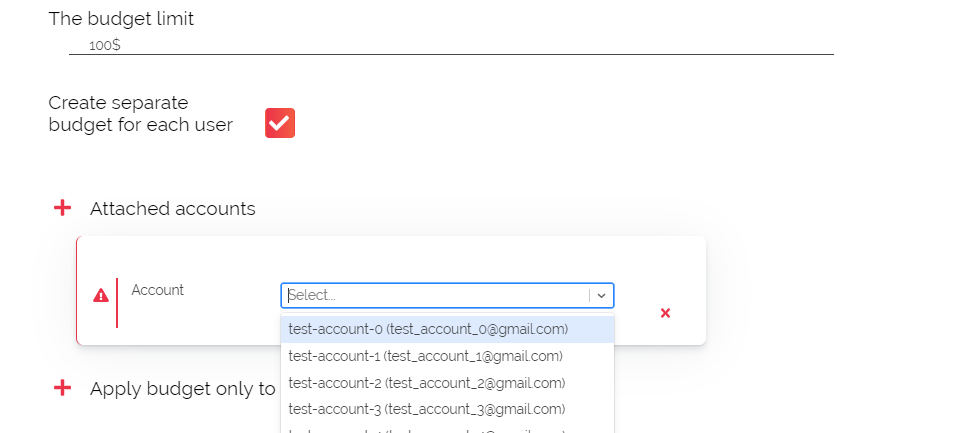
\includegraphics[width=\textwidth,height=200pt,keepaspectratio] {imgs/screenshots/screen_budgets_create.png}}
      \caption{The budget creation form\label{fig:scr-budget-create}}
    \end{figure}
    
    The budget listing (Figure 3.6) presents a visually simple grid with all reported and forecasted
    costs as well as comparison charts to quickly compare spendings.
    
    \begin{figure}[H]
      \center{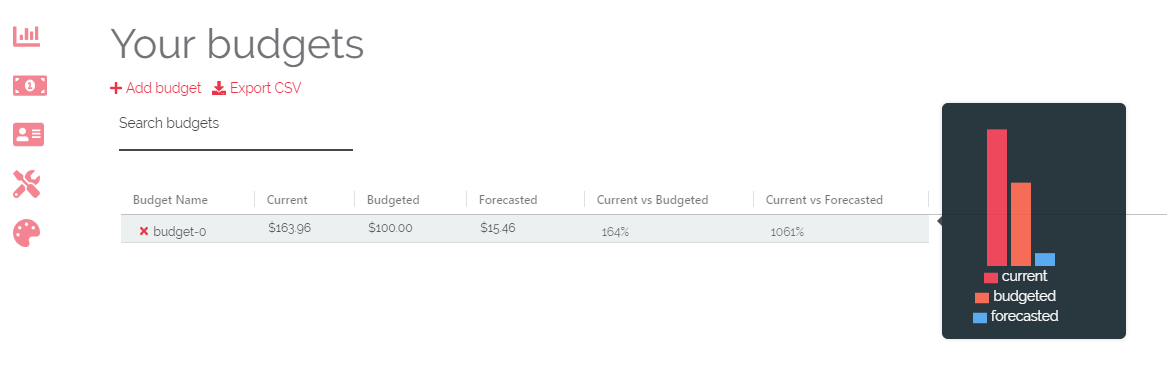
\includegraphics[width=\textwidth,height=200pt,keepaspectratio] {imgs/screenshots/screen_budgets_browse.png}}
      \caption{The budget browser\label{fig:scr-budget-browse}}
    \end{figure}
    
    \subsection{Accounts and user management}
    
    The account listing (Figure 3.7) allows users to browse all AWS accounts
    and presents useful details for each of them (i.e. ARN, IDs etc.).
    
    \begin{figure}[H]
      \center{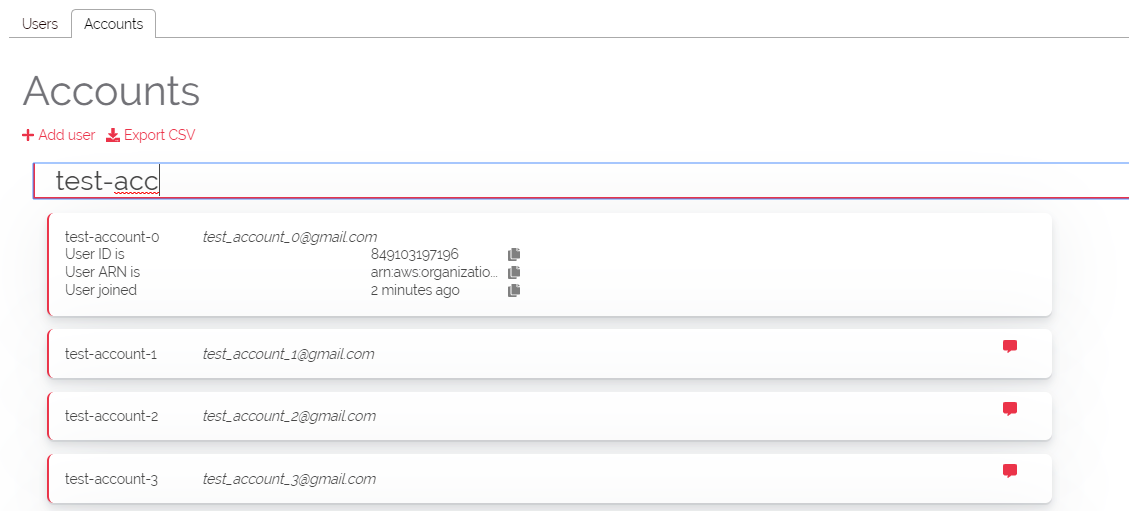
\includegraphics[width=\textwidth,height=200pt,keepaspectratio] {imgs/screenshots/screen_accounts_browse.png}}
      \caption{The account list view\label{fig:scr-account-browse}}
    \end{figure}
    
    The similar view exists in the users tab (Figure 3.8) to present all created user accounts in the system.
    
    \begin{figure}[H]
      \center{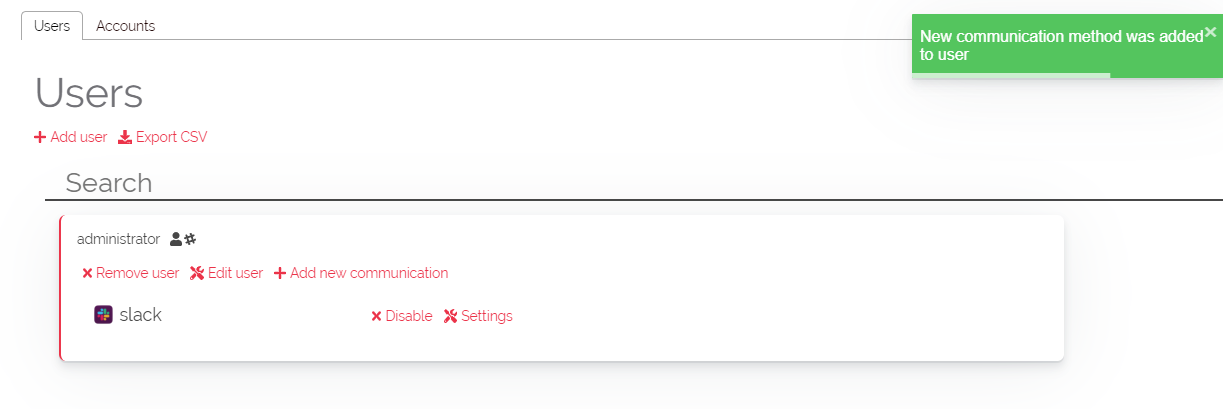
\includegraphics[width=\textwidth,height=200pt,keepaspectratio] {imgs/screenshots/screen_users_browse.png}}
      \caption{The user list view\label{fig:scr-user-browse}}
    \end{figure}
    
    Creation of the new user is a straightforward process.
    The user can, using views from Figures 3.8 and 3.9, easily:
    \begin{enumerate}
        \item Remove or attach new communication channels
          to the created users (i.e. connect Slack or email accounts to receive notifications).
        \item Remove or attach new accounts to the user
          (the user will be notified when these accounts will be overbudgeted).
        \item Delete users or change their properties.
    \end{enumerate}
    
    \begin{figure}[H]
      \center{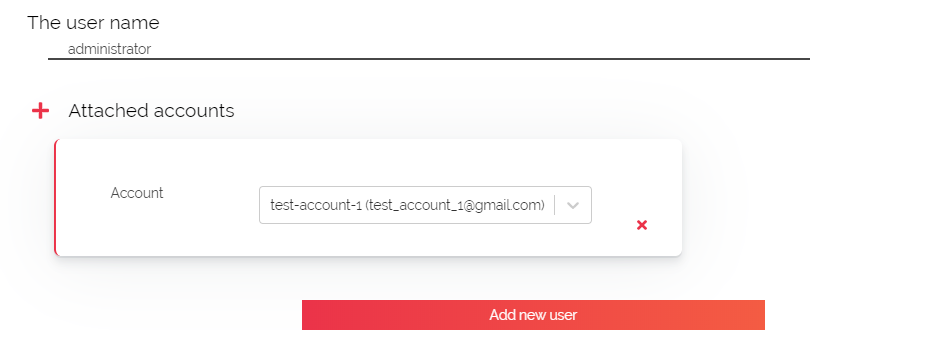
\includegraphics[width=\textwidth,height=200pt,keepaspectratio] {imgs/screenshots/screen_users_create.png}}
      \caption{The user creation form\label{fig:scr-user-create}}
    \end{figure}
    
    \subsection{Customization}
    
    The views responsible for managing various application settings
    were spread across configuration panels available for access
    from a central settings view (Figure 3.10) to allow users to easily change
    them without introducing a configuration option mess.
    
    \begin{figure}[H]
      \center{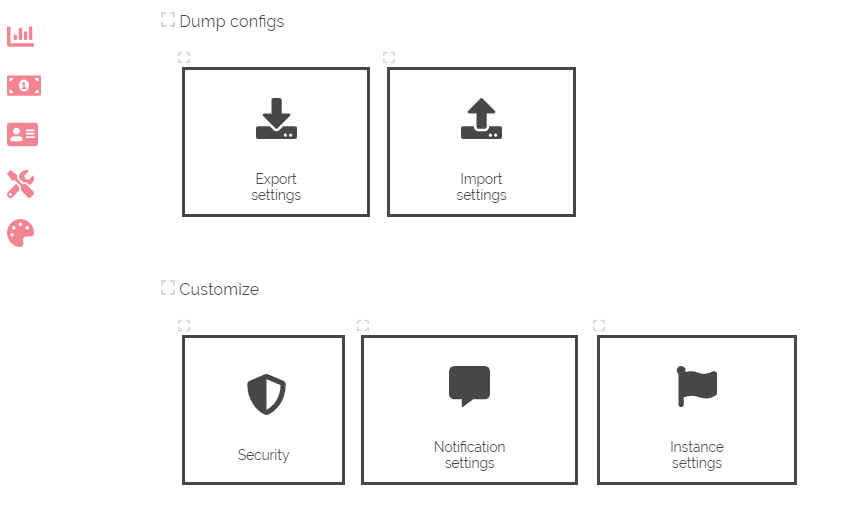
\includegraphics[width=\textwidth,height=200pt,keepaspectratio] {imgs/screenshots/screen_customize.png}}
      \caption{The settings view\label{fig:scr-customize}}
    \end{figure}
    
    Here the user can change:
    \begin{enumerate}
        \item enabled extensions and integrations (Figure 3.11),
        \item instance settings (i.e. AWS keys, deployment URLs etc.) (Figure 3.12),
        \item theming options to customize the look and feel of the application (Figure 3.13),
        \item current notification settings (Figure 3.14).
    \end{enumerate}
    
    The extension screens (Figure 3.11) allow users to enable or disable
    dashboard extensions (for example hide the budgets view if wanted) or change their settings.
    
    \begin{figure}[H]
      \center{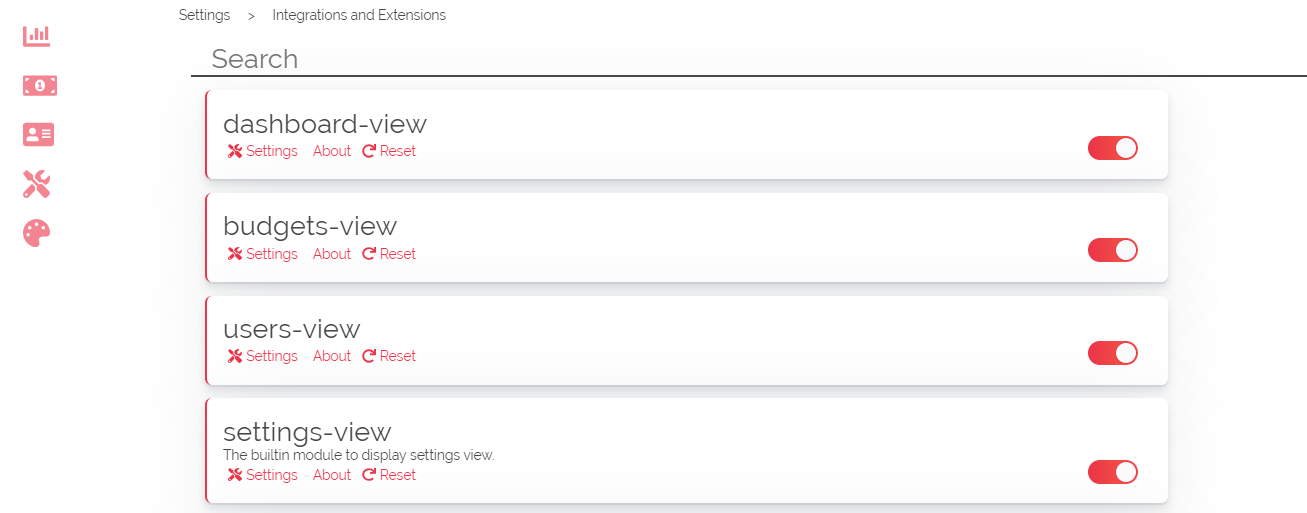
\includegraphics[width=\textwidth,height=200pt,keepaspectratio] {imgs/screenshots/screen_customize_extensions.png}}
      \caption{The view management panel\label{fig:scr-extensions}}
    \end{figure}
    
    The instance settings screen (Figure 3.12) is a straightforward way to manage
    Omigost deployment settings. You can provide your own services URLs for Omigost dependencies
    (like custom AWS Budgets store service) or change AWS and Slack credentials.
    
    \begin{figure}[H]
      \center{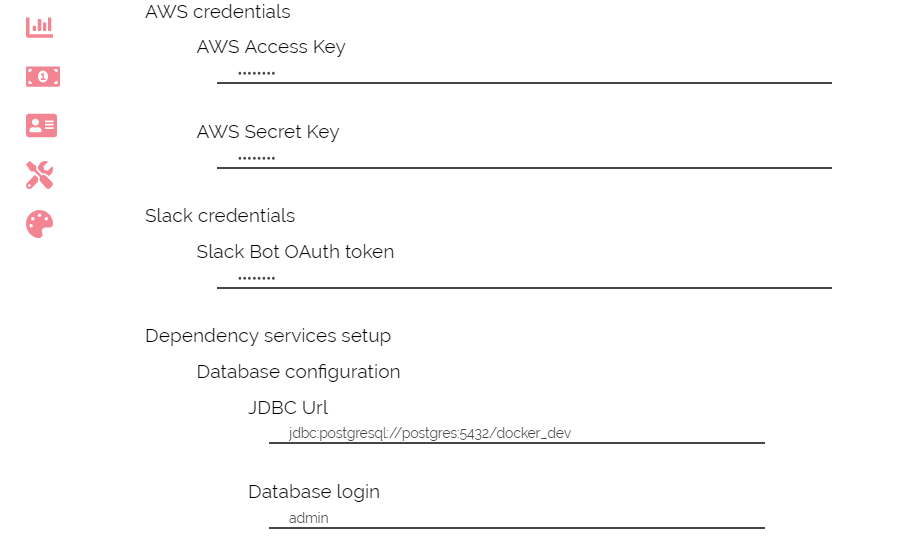
\includegraphics[width=\textwidth,height=200pt,keepaspectratio] {imgs/screenshots/screen_customize_settings.png}}
      \caption{The instance settings view\label{fig:scr-instance-settings}}
    \end{figure}
    
    Theming views (Figure 3.13) are useful to change the look and feel of the application
    to make users comfortable with a more friendly, customized environment.
    
    \begin{figure}[H]
      \center{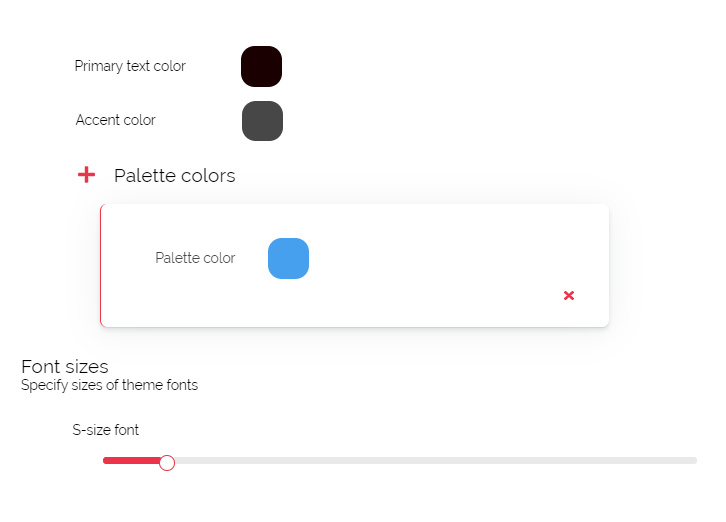
\includegraphics[width=\textwidth,height=200pt,keepaspectratio] {imgs/screenshots/screen_customize_theme.png}}
      \caption{Theme customization panel\label{fig:scr-theme}}
    \end{figure}

    Customization settings (Figure 3.14) allow the user to define the timeframe
    the system should consider for suggesting machine termination
    to the employees.

    \begin{figure}[H]
      \center{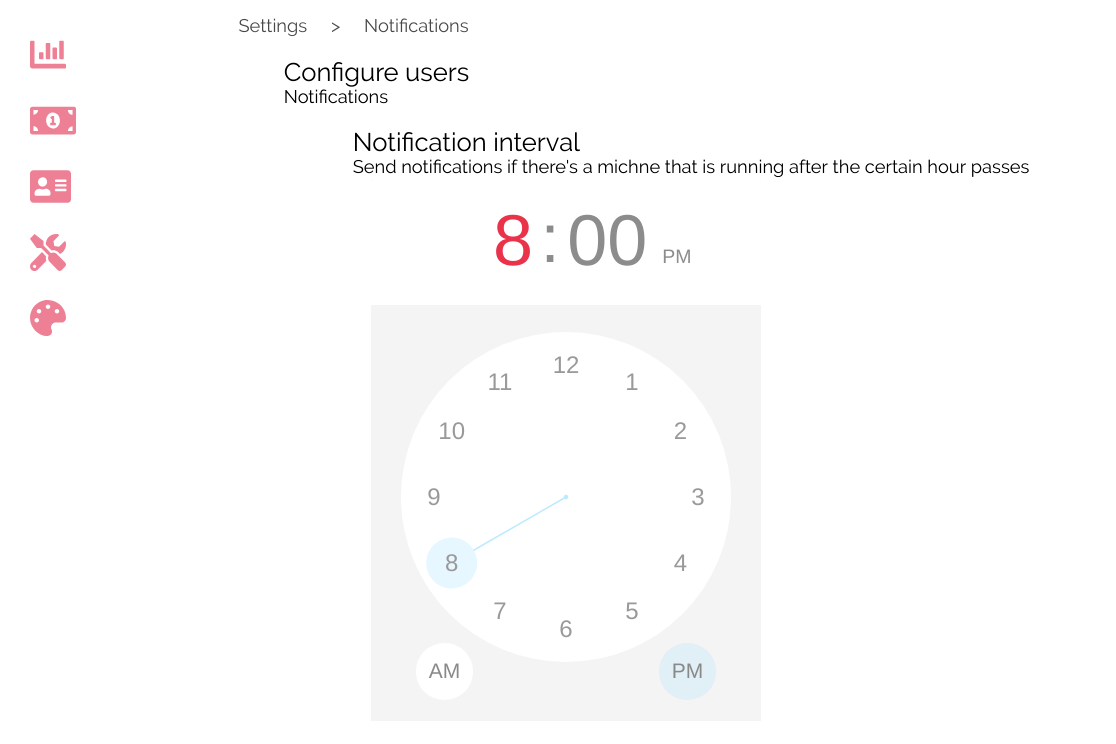
\includegraphics[width=\textwidth,height=200pt,keepaspectratio] {imgs/screenshots/screen_customize_notifications.png}}
      \caption{Notification customization panel\label{fig:scr-notify}}
    \end{figure}
    

    \section{Communication integration}
    The application is designed for two groups of users: the employees and the administrators.
    While the frontend interface we describe in section 3.4.1 is created mainly for the usage
    of the administrators, the interaction between the system and the employees is mostly
    handled via Slack.

    Slack collaboration workspaces allow to inject multiple functionalities
    in a form of Slack apps.
    Slack apps offer many customization and extension options, but to cover
    the needs of Omigost users we mainly had to rely on a bot feature
    that allows to message users.

    \subsection{Setup and configuration}

    Basically, to be able to use Omigost with Slack, first of all the administrator
    has to install an Omigost Slack app, choosing from a range of other apps
    available on Slack's app page.
    Alternatively, it is possible to set up the app on one's own
    in a Slack collaboration workspace.
    As a result, an Omigost bot capable of messaging users is added to the workspace.
    The administrator is then also provided with an API token that can be entered in
    the main Omigost server configuration for it to be able
    to connect to and use that bot.
    The administrator should then provide Slack usernames in the attached
    workspace for each user in a dedicated configuration panel.
    He also configures who among those users should be considered an administrator
    so the system can also notify him.

    \subsection{Messaging details}

    The integration itself is made possible thanks to the REST API
    that Slack exposes for each instance of a Slack app.
    Every time the app needs to send a message to a user, it issues HTTP
    calls that specify the message content, potential attachments and destination.

    To allow interactions with the system, messages issued by Omigost
    can contain either links or actions.
    We use links to route users to forms that they can fulfill
    to provide additional info to the system.
    The forms use short-lived, single-use generated tokens for identifying
    correlation between form payload and an event that this payload responds to.

    \subsection{Slack message use cases}

    The Slack bot sends notification to the users when they cross
    a predefined budget or leave instances running after the business hours.

    Budget notification flow is as follows: on an event of the system detecting
    either forecasting or detecting a budget overflow, the system collects
    a list of users responsible for machines that are related to that budget.
    To each of those users we send a message that contains actual or potential
    budget overflow details as well as a button link to a form where that user can request
    an increase to the budget limit.
    Responding via such a form results in the system notifying the administrators
    about a new limit increase request so they can then decide whether to comply
    with the request, and then act accordingly.

    Machine termination is suggested to the users with messages
    when bussiness hours of a day are nearing to an end.
    The messages tell the user how many machines are running at the moment
    and provides a set of actions that enable the user to conveniently stop
    or terminate them.
    After a successful teardown the user is also notified with a "Done!" message.

    The implementation of the machine termination communication has certain subtleties.
    Comparing to the budget messages, the application doesn’t keep track of messages
    related to machine termination, but
    only tracks the timestamps of the last time a person was notified via any channel.
    This allows us to limit the number of notifications and not spam the user.

    As the communication is asynchronous between the application and the end user,
    we do not rely on an immediate response.
    Instead, we bundle the message with the encrypted user AWS identifier
    and the timestamp of the notification.
    We also keep the encryption keys in the databases for the other instances
    of the application to be able to handle any request.
    The key-timestamp pairs help us identify the user, implement action timeout
    and make sure that nobody from the outside can stop the application
    on behalf of the users.
    Such an architecture helps us keep the application stateless
    and increases the overall security of the system.

    \section{Service termination architecture}
    While developing the application, we kept in mind a certain model
    of organizing the resources
    which the enterprise user might have in the AWS cloud.
    A common way of keeping an organization in AWS cloud
    is via a service called “AWS Organizations”~\cite{AWSOrganizations}.
    The service allows to allocate AWS accounts
    with predefined roles and permissions for every member of an organization.
    Such a structure also isolates resources from each other
    and lowers the granular control that the root account has on user allocated resources.

    For our application to be able to tweak and monitor every machine
    created by the organization members, every employee of the organization
    needs to create a certain predefined role
    which should have the same name across all accounts.
    The role should have access to all resources that the user wants to be monitored.
    This can be done by a simple script every time a new member joins the organization.

    Secondly, the owner of the account the application is being set up for
    needs to create an AWS IAM user~\cite{AWSIAM},
    which will be used by the application to assume
    the roles created by other members of the organization.
    To enable the functionality, the administrator needs
    to give an “AssumeRole” permission to the newly created IAM user.

    We recommend to take the following steps to grant the above-mentioned permission.


    \begin{enumerate}
        \item Create an IAM group called “AssumesRolesGroup”.
        \item Go to the permissions section of the group.
        \item Create a custom group policy.
        \item Add the following “JSON” to the policy document.

        \begin{lstlisting}[language=json,firstnumber=1]
        {
          "Version": "2012-10-17",
          "Statement": [
            {
              "Effect": "Allow",
              "Action": [
                "sts:AssumeRole"
              ],
              "Resource": "*"
            }
          ]
        }
        \end{lstlisting}

        \item Add the IAM user to the “AssumesRoleGroup” group.
    \end{enumerate}

    After taking all those steps, the user only has to copy
    the AWS keys of that IAM user account
    to the application configuration file to give the backend server
    an access to that permission grant.

    \chapter{Project development}

    In this chapter we describe the way we developed
    the application -- management and organization of work along with supporting tools.

    \section{Version control}

    During the development as our version control system we used Git
    and the whole code repository has been being hosted on GitHub.
    We have chosen this particular service because of a few reasons.

    First of all, GitHub~\cite{GitHub} is one of the most popular Git hosting services
    and also has one of the largest open source communities.
    This is quite important -- especially when considering a possibility of
    future development of the tool after finishing this thesis.

    The second reason is integration with lots of useful applications.
    It is easy to use it with different services that improve the development
    process, like TravisCI~\cite{TravisCI} and Slack~\cite{Slack}.

    Last but not least, GitHub has a built in issue tracker.
    It can be highly customised and makes project management easier.
    We created a dashboard divided into a few sections, which separate tasks
    in different stages of development.
    Everything has been automated -- depending on actions performed by users,
    like merging Pull Requests (PRs), issues have been being moved between sections.
    In order to help prioritize tasks we employed GitHub's issue tagging system.

    \section{Continuous Integration}

    For Continuous Integration we used a hosted service -- TravisCI.
    It allowed us to make sure new changes we introduce
    are compliant with the rest of our codebase.
    There are two reasons we have chosen this service:
    it is easy to configure using only one YAML file
    inside the repository and it is free for open source projects.
    After every code submission, at the beginning TravisCI
    has performed Smoke Tests, attempting to build the project
    and checking whether it runs or not.
    Successful build has been followed by both backend and frontend tests.

    \section{Communication}

    All of the communication has happened via Slack.
    It is a convenient collaboration platform allowing team members
    to communicate efficiently.
    Everybody can create their own instance of a Slack workspace and then
    invite other members to join and use it.
    Various channels can be created there,
    with persistent message history both public and private.
    There is also a possibility to reach out to any member directly whenever needed.
    Today Slack is one of the most popular options for groups of any kind to coordinate
    their teamwork on a daily basis.
    We have been using Slack because it is free, it integrates easily with GitHub
    and it has allowed us to test Omigost integration with Slack easily.

    \section{Organization of work}

    We have been working in iterations that lasted around one month.
    In the beginning, we defined and created new issues.
    During the iteration, everyone chose desirable task,
    then completed it and made a corresponding Pull Request in GitHub.
    In the end, we discussed our overall progress and planned next steps.

    In order to let a new feature become part of the repository it had to be accepted.
    It means that Pull Request had to pass Continuous Integration
    system build and be approved by one of the reviewers.
    Every issue was being solved in a separate branch and every PR
    was being merged directly to the master branch, which has allowed us
    to group all commits that has been a part of a single feature or issue.

    \section{Contact with the client company -- Sumo Logic}

    The whole project and the thesis has been developed under Sumo Logic mentorship.
    There has been one particular person designated to act as mentor -- Jacek Migdał.
    He made sure we are provided with every resource we needed to
    work on the project without unnecessary breaks.
    Also, our mentor helped revolve any ambiguity and gave technical advice.

    Day to day communication with mentor took place via Slack.
    Additionally, approximately twice a month our team has been meeting
    in the Sumo Logic office to review current progress and overcome major difficulties.
    Every new feature has been discussed beforehand with the company.

    \chapter{Summary}
    The purpose of the project was to implement a solution for optimizing cloud costs
    in a typical medium-sized company according to the needs reported by Sumologic.
    From two approaches that were suggested by the ordering party,
    we chose one that was more software-focused rather than analytic.

    Development spanned a period of about a half of a year and planning and preparations took us
    a few more months.
    We developed our application in irregular iterations that each of us adjusted
    to their schedule.
    Additionally, we held meetings with our supervisor roughly every 2-3 weeks
    as well as with the contractor when we needed to consult development and requirement details.
    The company expressed a huge interest in the implementation of the project
    as well as further development of it.

    In the end we built a system focusing on simplifying AWS Budgets management
    and machine termination automation,
    both of which benefit heavily from a Slack integration.

    The product is a web application consisting of Java Spring server
    and Typescript browser frontend.
    The solution is deployed along a Postgres relational database with a Docker container
    on a Beanstalk instance.
    The project is fully open-source, released under MIT license
    and available on GitHub~\cite{Omigost}.


    \begin{thebibliography}{99}
        \addcontentsline{toc}{chapter}{Bibliography}

        \bibitem[Apptio]{Apptio}
        Apptio, Inc. 2007-2019.
        \textit{Apptio Fuels Digital Transformation}.
        Apptio toolkit overview.
        \textit{https://www.apptio.com/products}.
        Accessed on 01 April 2019.

        \bibitem[Armbrust]{Armbrust}
        M. Armbrust, A. Fox, R. Griffith, A. D. Joseph, R. H. Katz et al. 2009.
        \textit{Above the Clouds: A Berkeley View of Cloud Computing}.
        Technical Report No. UCB/EECS-2009-28.
        \textit{http://www.eecs.berkeley.edu/Pubs/TechRpts/2009/EECS-2009-28.html}.

        \bibitem[AWSCostManagement]{AWSCostManagement}
        Amazon Web Services, Inc. or its affiliates. 2019.
        \textit{AWS Cost Management -- Welcome Page}.
        Initial description of the Cost Explorer and AWS Budgets API usage.
        \textit{https://docs.aws.amazon.com/aws-cost-management/latest/APIReference/Welcome.html}.
        Accessed on 01 April 2019.

        \bibitem[AWSDocs]{AWSDocs}
        Amazon Web Services, Inc. or its affiliates. 2019.
        \textit{AWS documentation}.
        \textit{https://docs.aws.amazon.com}.
        Accessed on 01 April 2019.

        \bibitem[AWSIAM]{AWSIAM}
        Amazon Web Services, Inc. or its affiliates. 2019.
        \textit{AWS Identity and Access Management (IAM) documentation}.
        \textit{https://docs.aws.amazon.com/iam/index.html}.
        Accessed on 01 April 2019.

        \bibitem[AWSOrganizations]{AWSOrganizations}
        Amazon Web Services, Inc. or its affiliates. 2019.
        \textit{AWS organizations documentation}.
        \textit{https://docs.aws.amazon.com/organizations/index.html}.
        Accessed on 01 April 2019.

        \bibitem[Cloudability]{Cloudability}
        Cloudability Inc. 2019.
        \textit{Cloudability - Platform Overview}.
        Cloudability frontpage, description of its capabilities.
        \textit{https://www.cloudability.com/product/}.
        Accessed on 01 April 2019.

        \bibitem[CloudabilityAlerts]{CloudabilityAlerts}
        Leah Weitz. 2015.
        \textit{Creating budget alerts by tag with Cloudability}.
        Blog entry about budget management with Cloudability tool.
        \textit{https://blog.cloudability.com/creating-budget-alerts-by-tag-with-cloudability/}.

        \bibitem[CostExplorer]{CostExplorer}
        Amazon Web Services, Inc. or its affiliates. 2019.
        \textit{AWS Cost Explorer}.
        Service Capabilities Description.
        \textit{https://aws.amazon.com/aws-cost-management/aws-cost-explorer/}.
        Accessed on 01 April 2019.

        \bibitem[Docker]{Docker}
        Docker Inc. 2019.
        \textit{Docker. Enterprise Container Platform for High-Velocity Innovation}.
        Docker tool frontpage.
        \textit{https://www.docker.com/}.
        Accessed on 23 May 2019.

        \bibitem[GitHub]{GitHub}
        GitHub, Inc. 2019.
        \textit{GitHub. Built for developers}.
        GitHub tool frontpage.
        \textit{https://github.com/}.
        Accessed on 23 May 2019.

        \bibitem[Gradle]{Gradle}
        Gradle Inc. 2019.
        \textit{Gradle Build Tool}.
        Gradle tool frontpage.
        \textit{https://gradle.org/}.
        Accessed on 18 June 2019.

        \bibitem[Laatikainen]{Laatikainen}
        G. Laatikainen, A. Ojala, O. Mazhelis. 2013.
        \textit{Cloud Services Pricing Models}.

        \bibitem[Markus]{Markus}
        M. Böhm, S. Leimeisier, C. Riedl, H. Krcmar. 2011.
        \textit{Cloud Computing and Computing Evolution}.
        Technische Universität München (TUM), Germany.

        \bibitem[Omigost]{Omigost}
        Omigost project.
        \textit{https://github.com/Omigost/}.
        Accessed on 18 June 2019.

        \bibitem[Project Lombok]{Project Lombok}
        The Project Lombok Authors. 2009-2019.
        \textit{Project Lombok}.
        Project Lombok library frontpage.
        \textit{https://projectlombok.org/}.
        Accessed on 01 April 2019.

        \bibitem[React]{React}
        Facebook Inc. 2019.
        \textit{React. A JavaScript library for building user interfaces}.
        React framework official frontpage.
        \textit{https://reactjs.org/}.
        Accessed on 23 May 2019.

        \bibitem[Slack]{Slack}
        Slack Technologies. 2019.
        \textit{Slack. Imagine what you’ll accomplish together}.
        Slack tool frontpage.
        \textit{https://slack.com/}.
        Accessed on 23 May 2019.

        \bibitem[SnowBlog]{SnowBlog}
        David Svee. 2017.
        \textit{The True Cost of AWS}.
        Overview of cloud cost issues and ways to optimize them.
        \textit{https://www.snowsoftware.com/es/blog/2018/06/16/true-cost-aws}.
        Accessed on 01 April 2019.

        \bibitem[SnowSaaS]{SnowSaaS}
        Snow Software. 2018.
        \textit{Snow for SaaS | Snow Software -- The Cloud Challenge}.
        Description of Snow for SaaS targets.
        \textit{https://www.snowsoftware.com/int/snow-saas}.
        Accessed on 01 April 2019.

        \bibitem[Spring]{Spring}
        Pivotal Software, Inc. 2019.
        \textit{Spring by Pivotal. The right stack for the right job}.
        Spring framework frontpage.
        \textit{https://spring.io/}.
        Accessed on 23 May 2019.

        \bibitem[Stax.io]{Stax.io}
        Stax.
        \textit{Stax. Empowering companies to build better cloud}.
        Stax.io tool frontpage, description of the tool.
        \textit{https://www.stax.io/}.
        Accessed on 23 May 2019.

        \bibitem[TravisCI]{TravisCI}
        Travis CI, GmbH. 2019.
        \textit{Travis CI. Test and Deploy with Confidence}.
        Travis CI Continuous Integration service frontpage.
        \textit{https://travis-ci.org/}.
        Accessed on 23 May 2019.

        \bibitem[Typescript]{Typescript}
        Microsoft. 2019.
        \textit{Typescript. JavaScript that scales}.
        Typescript language official webpage.
        \textit{https://www.typescriptlang.org/}.
        Accessed on 23 May 2019.

        \bibitem[UXPin]{UXPin}
        2019 UXPin Inc.
        \textit{UXPin}.
        UXPin tool official webpage.
        \textit{https://www.uxpin.com/}.
        Accessed - 28 May 2019.
        
    \end{thebibliography}

\end{document}


%%% Local Variables:
%%% mode: latex
%%% TeX-master: t
%%% coding: latin-2
%%% End:
